\documentclass{article}

\usepackage{amsmath,amssymb}
\usepackage{tikz}
\usepackage{pgfplots}
\usepackage{xcolor}
\usepackage[left=2.1cm,right=3.1cm,bottom=3cm,footskip=0.75cm,headsep=0.5cm]{geometry}
\usepackage{enumerate}
\usepackage{enumitem}
\usepackage{marvosym}
\usepackage{tabularx}

\usepackage{listings}
\definecolor{lightlightgray}{rgb}{0.95,0.95,0.95}
\definecolor{lila}{rgb}{0.8,0,0.8}
\definecolor{mygray}{rgb}{0.5,0.5,0.5}
\definecolor{mygreen}{rgb}{0,0.8,0.26}
\lstdefinestyle{java} {language=java}
\lstset{language=java,
	basicstyle=\ttfamily,
	keywordstyle=\color{lila},
	commentstyle=\color{lightgray},
	stringstyle=\color{mygreen}\ttfamily,
	backgroundcolor=\color{white},
	showstringspaces=false,
	numbers=left,
	numbersep=10pt,
	numberstyle=\color{mygray}\ttfamily,
	identifierstyle=\color{blue},
	xleftmargin=.1\textwidth, 
	%xrightmargin=.1\textwidth,
	escapechar=§,
	breaklines=true,
	postbreak=\mbox{\space}
}

\usepackage[utf8]{inputenc}

\renewcommand*{\arraystretch}{1.4}

\newcolumntype{L}[1]{>{\raggedright\arraybackslash}p{#1}}
\newcolumntype{R}[1]{>{\raggedleft\arraybackslash}p{#1}}
\newcolumntype{C}[1]{>{\centering\let\newline\\\arraybackslash\hspace{0pt}}m{#1}}

\newcommand{\E}{\mathbb{E}}
\DeclareMathOperator{\rk}{rk}
\DeclareMathOperator{\Var}{Var}
\DeclareMathOperator{\Cov}{Cov}

\title{\textbf{Softwaretechnologie, Übung 7}}
\author{\textsc{Henry Haustein}}
\date{}

\begin{document}
	\maketitle
	
	\section*{Aufgabe 1}
	\begin{enumerate}[label=(\alph*)]
		\item kein gleichzeitiges Abspielen, nur eine Instanz des des AudioClipManagers (realisiert durch privaten Constructor)
		\item Singleton
		\item UML-Diagramm
		\begin{center}
			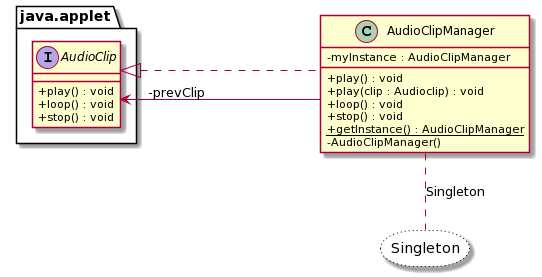
\includegraphics[width=0.75\textwidth]{./Aufgabe7_1}
		\end{center}
	\end{enumerate}

	\section*{Aufgabe 2}
	\begin{enumerate}[label=(\alph*)]
		\item FactoryMethod, Strategy
		\item UML-Diagramm
		\begin{center}
			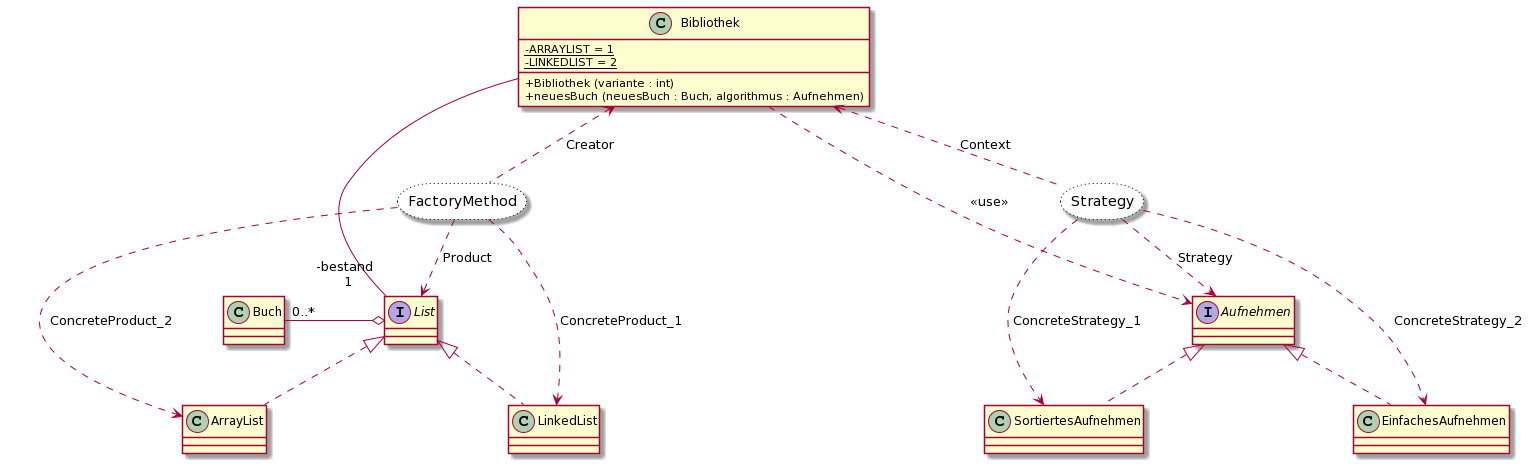
\includegraphics[width=0.94\textwidth]{./Aufgabe7_2}
		\end{center}
	\end{enumerate}

	\section*{Aufgabe 3}
	\begin{enumerate}[label=(\alph*)]
		\item TemplateMethod
		\item UML-Diagramm
		\begin{center}
			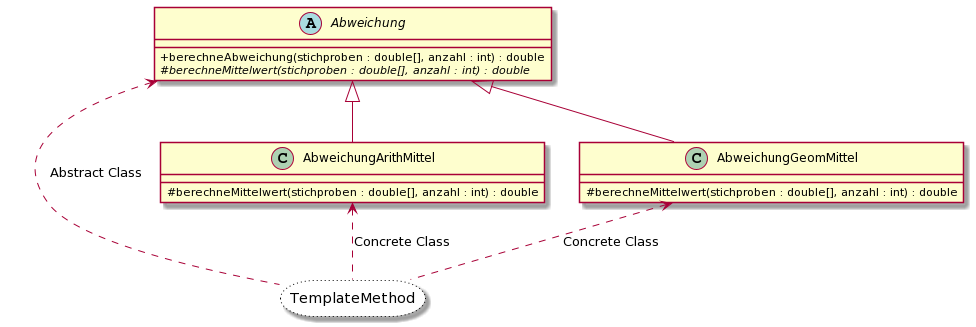
\includegraphics[width=1\textwidth]{./Aufgabe7_3}
		\end{center}
	\end{enumerate}
	
	\section*{Aufgabe 4}
	\begin{enumerate}[label=(\alph*)]
		\item UML-Diagramm für den ObjectAdapter
		\begin{center}
			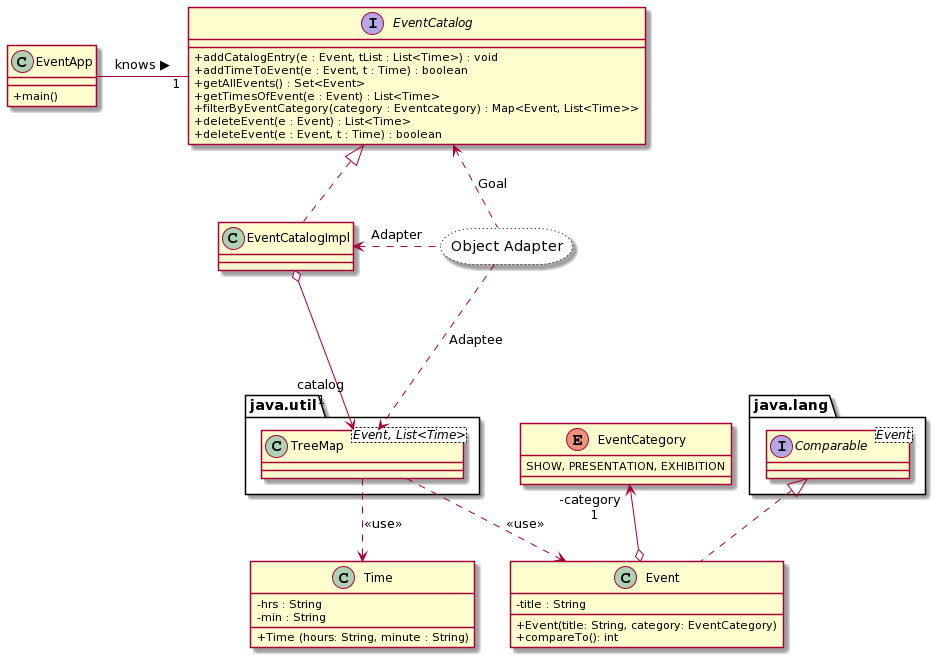
\includegraphics[width=0.95\textwidth]{./Aufgabe7_4a}
		\end{center}
		Implementierung
		\begin{lstlisting}[style=java, tabsize=2]
class EventApp {
	public static void main(String args[]) {
		EventCatalog eventCatalog = new EventCatalogImpl();
		Set<Event> allEvents = eventCatalog.getAllEvents();
	}
}

interface EventCatalog {
	public Set<Event> getAllEvents();
}

class EventCatalogImpl implements EventCatalog {
	Map<Event, List<Time>> catalog = new TreeMap<>();
	
	public Set<Event> getAllEvents() {
		return catalog.keySet();
	}
}
		\end{lstlisting}
		\item UML-Diagramm für den Klassenadapter
		\begin{center}
			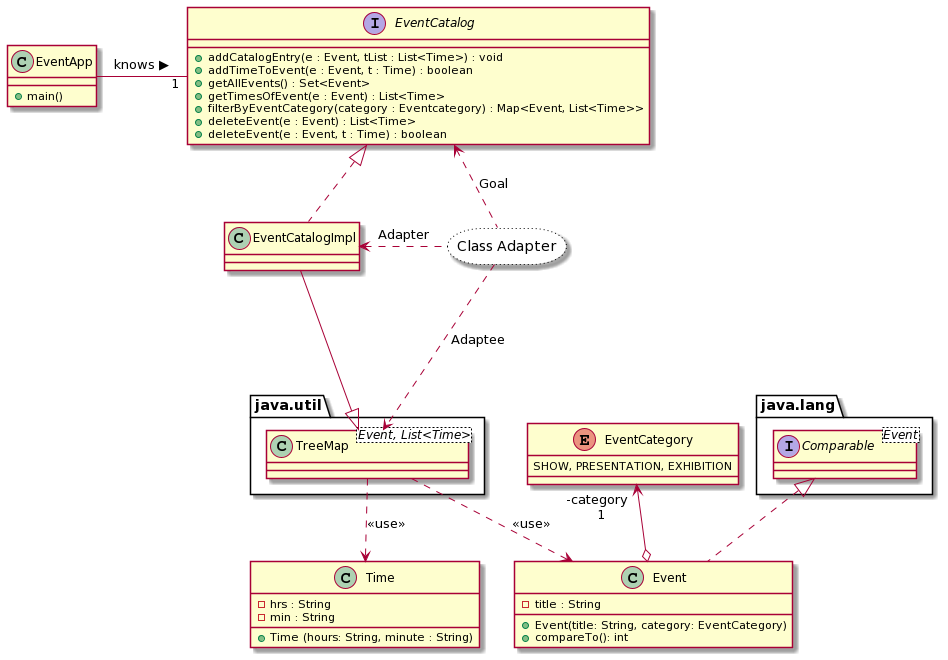
\includegraphics[width=0.95\textwidth]{./Aufgabe7_4b}
		\end{center}
		Implementierung
		\begin{lstlisting}[style=java, tabsize=2]
class EventApp {
	public static void main(String args[]) {
		EventCatalog eventCatalog = new EventCatalogImpl();
		Set<Event> allEvents = eventCatalog.getAllEvents();
	}
}

interface EventCatalog {
	public Set<Event> getAllEvents();
}

class EventCatalogImpl implements EventCatalog extends TreeMap<Event, List<Time>> {
	public Set<Event> getAllEvents() {
		return keySet();
	}
}
		\end{lstlisting}
	\end{enumerate}
\end{document}